\documentclass{beamer}
\usepackage{subcaption}
\usetheme{metropolis}

\usepackage{algorithm}
\usepackage[noend]{algpseudocode}

\title{Gaussian Processes for Data-Efficient Learning in Robotics and Control}
\subtitle{by Deisenroth, Fox, Rasmussen; pres. by Emmanuel Sales}
\date{2020-12-02}

\begin{document}
\begin{frame}
	\maketitle
\end{frame}	
\begin{frame}{Context}
	
	We want to \textbf{learn complex dynamics models} to achieve an optimal policy $\pi(x) = u$ for reaching a target state.
	
	\begin{itemize}
		\item Reinforcement learning: based on repeated trials, exploration, reward evaluations.
		\begin{itemize}
			\item Problem: RL is very slow, with a lot of data that needs to be collected for even simple problems.
		\end{itemize}
		\item Model-based methods could help with efficiency problems by providing additional information about the system.
		\begin{itemize}
			\item Problem: model-based methods are subject to uncertainty, and assuming that uncertainty away isn't going to produce good results.
		\end{itemize}	
	\end{itemize}
\end{frame}
\begin{frame}{Enter PILCO}
	PILCO (Probabilistic Inference for Learning Control) is a model-based policy search method.
	\begin{itemize}
		\item Based on Gaussian processes and gradient-based policy optimization. GPs allow modelling of uncertainty for each possible input point.
		\item Computationally efficient deterministic inference that's more \textbf{data-efficient} than the existing RL methods.
	\end{itemize}
\end{frame}
\begin{frame}{PILCO framework and Gaussian process overview}
	PILCO is based on \textbf{taking training input data} and \textbf{learning optimal GP models based on them}.
	
	Very general dynamical system model $$ x_{t+1} = f(x_t, u_t) + w, \quad w \sim \mathcal{N}(0, \Sigma_w) $$
	
	
\end{frame}
\begin{frame}{Gaussian process introduction}
	A GP is specified by a \textit{mean function} $m(z)$ and a \textit{covariance kernel} $k(z_1, z_2)$. For every $z$ in the domain of our function we model our function by $$ f(z) \sim \mathcal{N}(m(z), \Sigma_k(z, Z)) $$
	
	In PILCO our input space is both state and control space $\tilde{x} = (x,u) \in \mathbb{R}^{D + F}$ and they use the kernel $$ k(\tilde{x}_p, \tilde{x}_q) = \sigma_f^2 \exp\left(-\frac{1}{2}(\tilde{x}_p - \tilde{x}_q)^T \Lambda^{-1} (\tilde{x}_p - \tilde{x}_q)\right) + \delta_{pq} \sigma_w^2 $$
	
	GPs are trained in a Bayesian manner: the mean function and covariance matrix are updated as you feed the model training data ($Z$).
	
\end{frame}
\begin{frame}{Gaussian processes visualized}
	\begin{figure}[h]
		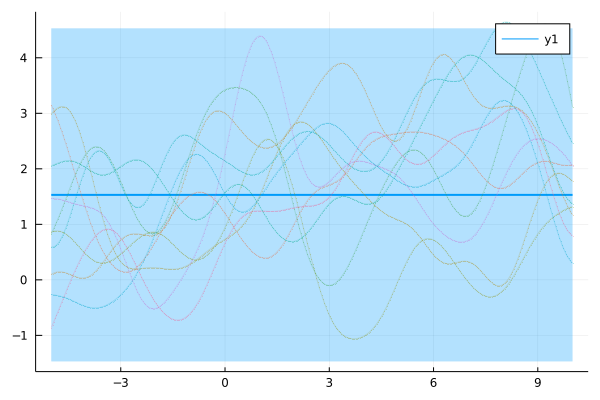
\includegraphics[width=200px]{./gp1_prior.png}
		\caption{example of a "prior" Gaussian process (before training). This includes 10 samples of the function.}
	\end{figure}
\end{frame}
\begin{frame}{Gaussian processes visualized}
	\begin{figure}[h]
		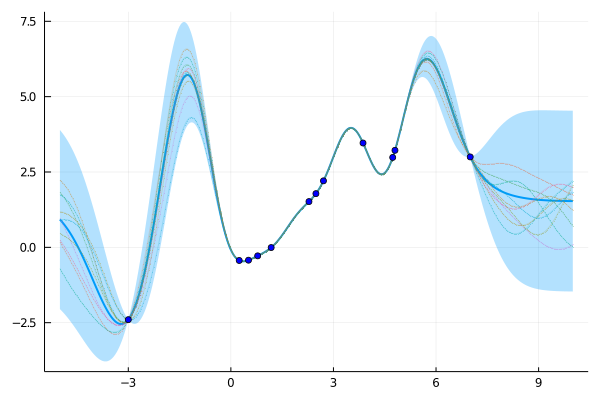
\includegraphics[width=200px]{./gp1.png}
		\caption{example of a "posterior" Gaussian process (after training). Notice that areas far away from training points have high variance, function at and near training points has very low variance}
	\end{figure}
\end{frame}
\begin{frame}{Gaussian Processes in PILCO prediction model}
	
	We form a general one-step GP-based prediction model between $x_t, u_t$ and $x_{t+1}$.
	
	For PILCO we have the following dynamics model: 
	
	$$ \mu_{t+1} = x_t + \mathbb{E}[\Delta_t], \quad \Sigma_{t+1} = \text{Var}_{f}[\Delta_t] $$
	
	Values of the GP at $\tilde{x}_t = (x_t, u_t)$ are inferred via conditional Gaussian laws and training data $\tilde{X}, y$: 
	
	$$ \mathbb{E}_f[\Delta_t] = m_f(\tilde{x}_t) = k(\tilde{X}, \tilde{x_t})^T(K(\tilde{X}) + \sigma^2_w I)^{-1}y$$
	
	$$ \text{Var}_f[\Delta_t] = k(\tilde{x}_t, \tilde{x}_t) - k(\tilde{X}, \tilde{x}_t)^{T}(K(\tilde{X}) + \sigma_w^2 I)^{-1} k(\tilde{X}, \tilde{x_t}) $$
	
	
	
\end{frame}
\begin{frame}{PILCO: policy iteration}
	Given our one-step prediction model, PILCO then needs to search for a parameterized \textit{policy} $\pi(x, \theta)$ that minimizes the expected long term cost
	
	$$ J^{\pi}(\theta) = \sum_{t=0}^{T} \mathbb{E}_{x_t}[c(x_t)], \quad x_0 \sim \mathcal{N}(\mu_0, \Sigma_0) $$
	
	$\theta$ are parameters of the policy, for a simple example take PID coefficients.
\end{frame}
\begin{frame}{Long-term predictions}
	
	To calculate $J^\pi$ we need to iteratively compute $p(x_1|\theta), \ldots, p(x_T|\theta)$.
	
	$$ p(x_{t+1}|\theta) = \iiint p(x_{t+1}|x_t, u_t) p(x_t, u_t|\theta) df dx_t du_t $$
	
	Problem: especially over longer time horizons, this distribution is very hard to compute. 
\end{frame}
\begin{frame}{Gaussian approximations}
	\begin{figure}[h]
		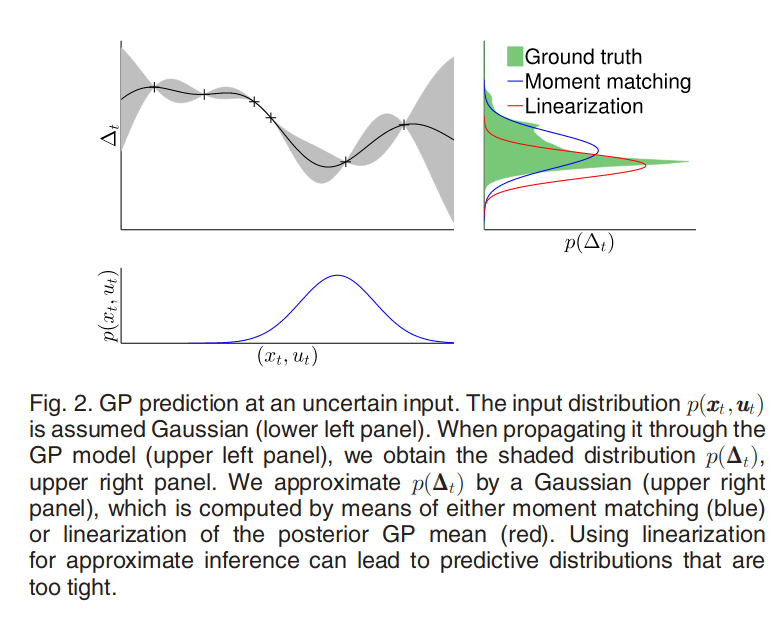
\includegraphics[width=120px]{./approx.png}
	\end{figure}
	We use Gaussian approximation on each time step in order to make the computation tractable. Two approaches for doing this:
	
	\begin{itemize}
		\item Moment matching - assume joint Gaussianity between input and prediction, compute mean and covariance of predictive distribution in closed form
		\item Linearization - linearize the nonlinear GP function at the mean of the input distribution
	\end{itemize}
	
	End up with Gaussian distributions for each time step over states and hence can calculate $\mathbb{E}[c(x_t)]$ for each $t$!
\end{frame}
\begin{frame}{Policy improvement}
	We now need to improve the policy. Calculate gradients $\frac{\partial J^{\pi}(\theta)}{\partial \theta}$ of the policy.
	
	$$ \frac{d J^{\pi}}{d \theta} = \sum_{t=1}^{T} \frac{d \mathbb{E}[c_t] }{d \theta} $$ and so forth... (very long chain)
	
	Afterwards, use a method like gradient descent or BFGS to find the optimum $\theta$.
\end{frame}
\begin{frame}{PILCO summary}
	High level version of the algorithm:
	\begin{algorithm}[H]
	\begin{algorithmic}[1]
		\Procedure{PILCO}{initial parameter $\theta_0$, input data $x$}
		\Repeat
			\State learn GP dynamics model using all data
			\Repeat
				\State Calculate approximated $J^\pi (\theta)$
				\State Improve policy using a gradient method based on $dJ(\theta) / d \theta$
			\Until{convergence; return $\theta^{*}$}
			\State $\pi^{*} \gets \pi(\theta^{*})$
			\State Apply $\pi^{*}$ to system and record data
		\Until{Task learned}
		\EndProcedure
		\end{algorithmic}
	\end{algorithm}
\end{frame}
\begin{frame}{Experimental results}
	
	\begin{minipage}{0.70\textwidth}
	\begin{itemize}
		\item Two tasks explored in small dimensions:
		\begin{itemize}
			\item Double pendulum swing-up (control space dimension $2$, state space $4$): after 50s, 95\% success rate
			\item Cart pole swing-up (control space $1$, state space $4$): after 15-20s, 95\% success rate
		\end{itemize} 
		\item Tested both moment matching ($O(n^2E^2D)$) and linearization ($O(n^2 ED)$) approximation techniques (MM was found to be more accurate)
	\end{itemize}
	\end{minipage}
	\begin{minipage}{0.25\textwidth}
		\begin{figure}[t]
			\begin{subfigure}{\linewidth}
				\centering
				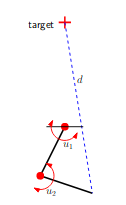
\includegraphics[width=0.9\linewidth]{./double_pendulum.png}
			\end{subfigure}

		\end{figure}
	\end{minipage}
\end{frame}
\begin{frame}{Comparison with other methods}
	\begin{minipage}{0.5\textwidth}
		\begin{itemize}
			\item Compared PILCO learning speed (data efficiency with other RL methods) including some that utilized learned dynamics models.
			\item PILCO outperforms any then-existing RL algorithm by at least one order of magnitude on cart-pole.
		\end{itemize}
	\end{minipage}\hfill
	\begin{minipage}{0.45\textwidth}
	\begin{figure}[H]
		\centering
		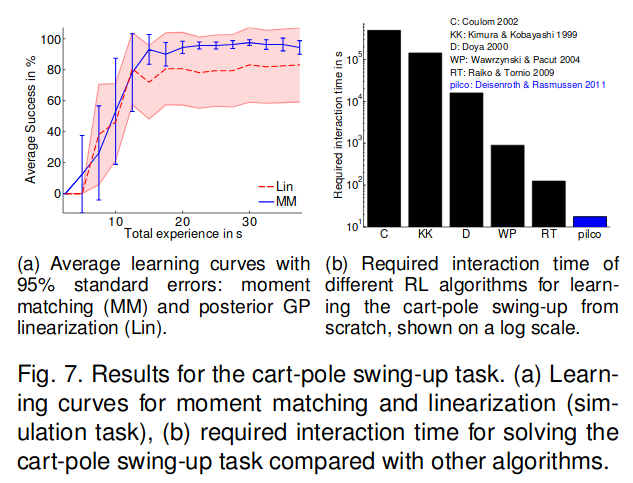
\includegraphics[width=\linewidth]{./results_chart.png}
	\end{figure}
	\end{minipage}
\end{frame}
\begin{frame}{Expanded experiments}
	\begin{minipage}{0.5\textwidth}
		\begin{itemize}
			\item Expanded to a higher dimension unicycle upright task (control space $2$, state space $12$), successful after 20 trials (30s)
			\item Expanded to hardware tasks for cart-pole swing up and robotic manipulator arm (no pose feedback, just visual feedback).
		\end{itemize}
	\end{minipage}\hfill
	\begin{minipage}{0.5\textwidth}
		\begin{figure}[ht]
			\begin{subfigure}{0.7\textwidth}
				\centering
				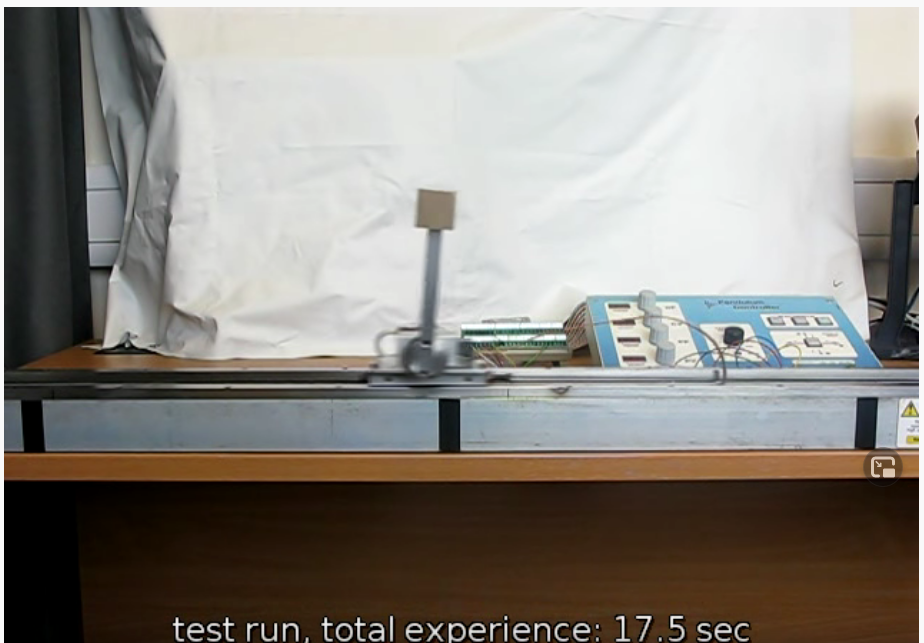
\includegraphics[width=\linewidth]{./cartpole_hardware.png}
			\end{subfigure}
			\begin{subfigure}{.5\textwidth}
				\centering
				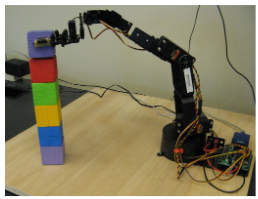
\includegraphics[width=\linewidth]{./manipulator.png}
			\end{subfigure}
		\end{figure}
	\end{minipage} 
	\begin{minipage}{\textwidth}
		\centering
		https://www.youtube.com/user/PilcoLearner
	\end{minipage}
\end{frame}
\begin{frame}{Deeper discussion}
	
	\begin{figure}
		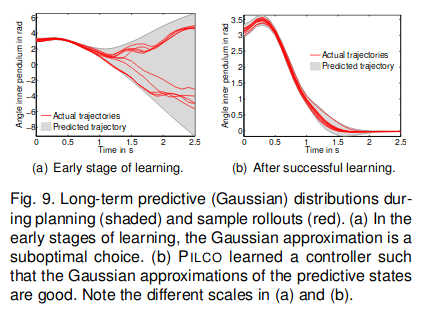
\includegraphics[width=0.5\textwidth]{./paper_fig9.png}
	\end{figure}
	
	\begin{itemize}
		\item Cost function (section 6) - unorthodox cost function that encourages exploration.
		\item Quality of Gaussian approximation (section 7) - how good is our assumption of Gaussian approximation? 
	\end{itemize}
\end{frame}
\begin{frame}{Conclusion}
	\begin{itemize}
		\item PILCO is a model-based learning framework that uses Gaussian processes to account for model uncertainty. It is a reinforcement learning approach that is able to learn in a data-efficient manner.
		\item Final line of the paper: "nonparametric Bayesian models can play a fundamental role in classical control setups, while avoiding the typically excessive reliance on explicit models"
	\end{itemize}
\end{frame}
\end{document}
